\chapter{پیاده‌سازی}
در بخش قبلی معماری کلی سیستم و ماژول‌های موردنیاز برای پیاده‌سازی سیستم ردیابی را بیان و به صورت اجمالی معرفی کردیم. در این فصل به چگونگی قرار گرفتن و ارتباط بخش‌های مختلف می‌پردازیم و پیاده‌سازی سیستم را توضیح خواهیم داد.


سیستم ردیابی طراحی شده در این پروژه از ماژول \lr{Arduino uno} و ماژول \lr{SIM808} که شامل آنتن \lr{GSM} و \lr{GPS} می‌باشد، برای ردیابی استفاده می‌کند. هسته اصلی این پروژه میکروکنترلر آردوینو می‌باشد. موقعیت جغرافیایی شی تویط آنتن \lr{GPS} دریافت شده و سپس این اطلاعات با استفاده از تکنولوژی \lr{GSM} به وب سرور فرستاده می‌شود. برای مشاهده کردن و ردیابی شی بر روی نقشه، یک برنامه کاربردی تحت وب توسعه داده شده است. این برنامه کاربردی به زبان \lr{PHP}، \lr{HTML} نوشته شده و از نرم‌افزار \lr{WampServer} برای اجرای آن استفاده می‌شود.
 
 
در ابتدا ماژول \lr{Sim808} برای گرفتن موقعیت مکانی از ماهواره مقداردهی اولیه می‌شود. تنظیمات اولیه این دستگاه با استفاده از دستورات \lr{AT} انجام می‌شود. با متصل کردن آنتن \lr{GPS} این ماژول قادر خواهد بود مختصات مکانی را از ماهواره دریافت کند. سپس تنظیمات مربوط به شبکه \lr{GPRS} انجام می‌شود.


آنتن‌های \lr{GSM} و \lr{GPS} به ماژول \lr{SIM808} متصل می‌شوند. برد آردوینو و ماژول \lr{SIM808} دارای پین اتصال به زمین مشترک هستند. برنامه نوشته شده به زبان \lr{C} بر با استفاده از نرم‌افزار \lr{Arduino IDE} روی برد آردوینو آپلود می‌شود.
\\
در شکل ۴-۱ نحوه اتصال ماژول‌های مختلف در سیستم ردیابی نشان داده شده است:
\begin{figure}[!h]
	\centerline{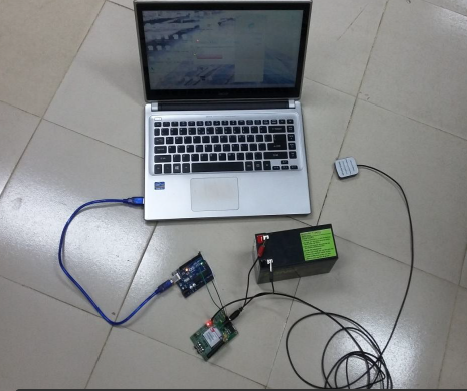
\includegraphics[width=.6\textwidth]{design-system}}
	\caption{سیستم ردیابی طراحی شده}
\end{figure}

